%%%%%%%%%%%%%%%%%%%%%%%%%%%%%%%%%%%%%%%%%%%%%%%%%%%%%%%%%%%%%%%%%%%%%
% LaTeX Template: Project Titlepage Modified (v 0.1) by rcx
%
% Original Source: http://www.howtotex.com
% Date: February 2014
% 
% This is a title page template which be used for articles & reports.
% 
% This is the modified version of the original Latex template from
% aforementioned website.
% 
%%%%%%%%%%%%%%%%%%%%%%%%%%%%%%%%%%%%%%%%%%%%%%%%%%%%%%%%%%%%%%%%%%%%%%

\documentclass[12pt]{article}
\usepackage[a4paper]{geometry}
\usepackage[myheadings]{fullpage}
\usepackage{fancyhdr}
\usepackage{lastpage}
\usepackage{graphicx, wrapfig, subcaption, setspace, booktabs}
\usepackage[T1]{fontenc}
\usepackage[font=small, labelfont=bf]{caption}
\usepackage{fourier}
\usepackage[protrusion=true, expansion=true]{microtype}
\usepackage[english]{babel}
\usepackage{sectsty}
\usepackage{url}
\usepackage{lmodern}
\usepackage[utf8]{inputenc}
\usepackage{varioref}
\usepackage {tikz}
\usepackage{float}
\usetikzlibrary {positioning}
\usetikzlibrary{calc}

\definecolor{DarkGreen}{RGB}{0,140,0}
\definecolor{DarkBlue}{RGB}{0,0,160}
\definecolor{DarkRed}{RGB}{220,0,0}
\definecolor{DarkPurple}{RGB}{160,0,160}



\newcommand{\HRule}[1]{\rule{\linewidth}{#1}}
\onehalfspacing
\setcounter{tocdepth}{5}
\setcounter{secnumdepth}{5}

%-------------------------------------------------------------------------------
% HEADER & FOOTER
%-------------------------------------------------------------------------------
\pagestyle{fancy}
\fancyhf{}
\setlength\headheight{15pt}
\fancyhead[L]{Algorithmique Appliquée}
\fancyhead[R]{L. Giovannangeli, F. Jacques, J. Narboni}
\fancyfoot[R]{Page \thepage\ of \pageref{LastPage}}
%-------------------------------------------------------------------------------
% TITLE PAGE
%-------------------------------------------------------------------------------

\begin{document}

\title{ \normalsize \textsc{Algorithmique Appliquée}
		\\ [2.0cm]
		\HRule{0.5pt} \\
		\LARGE \textbf{\uppercase{Projet RoboCup}}
		\HRule{2pt} \\ [0.5cm]
		\normalsize \today \vspace*{5\baselineskip}}

\date{}

\author{
		Loann Giovannangeli, Fabien Jacques, Jonathan Narboni}

\maketitle
\renewcommand{\contentsname}{Sommaire}
\newpage
\tableofcontents
\newpage

%-------------------------------------------------------------------------------
% Section title formatting
\sectionfont{\scshape}
%-------------------------------------------------------------------------------

%-------------------------------------------------------------------------------
% BODY
%-------------------------------------------------------------------------------
\part{Modélisation du Problème}

L'objectif de ce projet est de trouver une modélisation du problème de défense d'un but lors de la ligue SSL de la RoboCup et de l'implémenter. Ce problème consiste à trouver une manière optimale de placer les défenseurs par rapports à l'emplacement de leur but et des attaquants. Nous modéliserons le problème par un graphe. Une solution du problème sera un ensemble dominant de ce graphe.


\section{Entrées}
Les entrées de notre problème sont les informations qui nous intéressent sur nos robots et le terrain. Elles nous permettront de simuler la réalité dans nos algorithmes afin que nos résultats aient un sens concret.\\

Soient :
\begin{itemize}
\item $o_i \in O$ ($i \in \{1,..., n\}$) Les $n$ adversaires. On notera $o_i.x$ et $o_i.y$ les coordonnées de $o_i$.
\item $d_i \in D$ ($i \in \{1,..., k\}$) Les $m$ défenseurs.
\item $\theta_{step}$ Pas de discrétisation pour les angles de tirs. On considérera "l'angle $k$" comme étant un angle de mesure $k \cdot \theta_{step}$ radians. On nommera $K_{max}$ le plus grand angle possible, c'est à dire :  $\left \lfloor{\frac{2\cdot p \cdot i }{\theta_{step}}}\right \rfloor $
\item $pos_{step}$, $X_{min}$, $X_{max}$, $Y_{min}$, $Y_{max}$, Pas de discrétisation pour les positions sur le terrain, Abscisses et Ordonnées minimales et maximales.
\end{itemize}

\section{Fonctions nécessaires}
\begin{itemize}
\item $cadre(x, y, k)$ ($x, y, k \in N$) Fonction qui renvoie vrai si le tir d'un attaquant aux coordonnées $(x, y)$ d'angle $k$ est bien cadré et faux sinon.
\item $interception(x, y, k, x', y')$ Fonction qui renvoie vrai si le tir d'un attaquant en (x, y) d'angle k est arrêté par un défenseur en (x', y') et faux sinon.
\end{itemize}
\space
\space

\section{Graphe} \bigbreak
On crée le graphe G suivant :\\
\begin{figure}[H]
	\centering
	\scalebox{1.3}
	{
		
		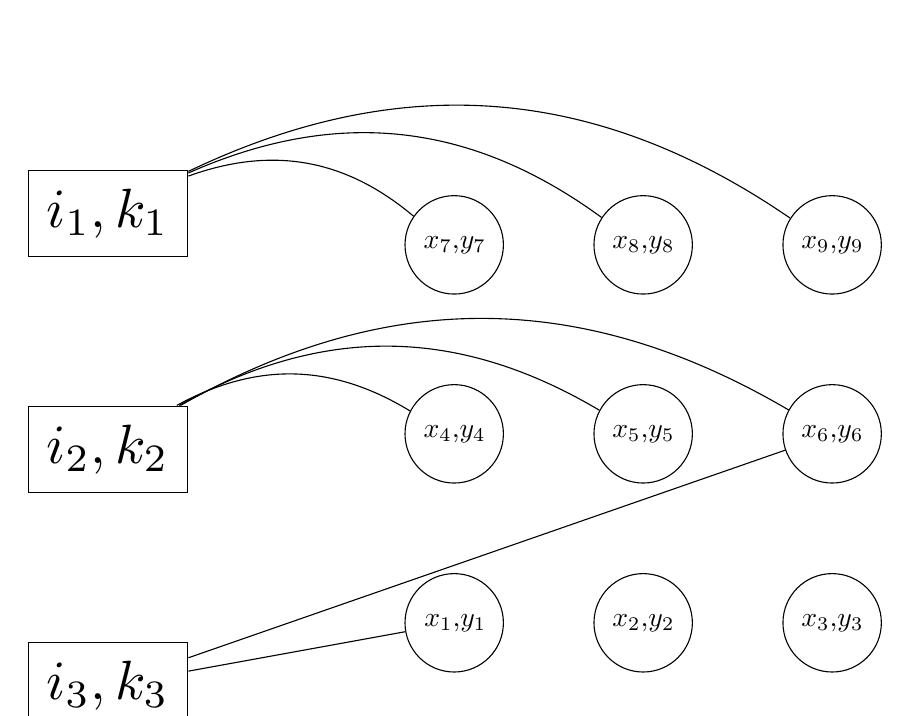
\begin{tikzpicture}[scale=2, transform shape,atq node/.style={shape=rectangle,scale=1,draw=black},def node/.style={scale=0.5, shape=circle,draw=black,inner sep=0,text width=35,align=center}, ]
		\node[atq node] (atq1) at (0,0){$i_3,k_3$};
		\node[atq node] (atq2) at (0,1.5){$i_2,k_2$};
		\node[atq node] (atq3) at (0,3){$i_1,k_1$};
		\newcounter{nDef};
		\setcounter{nDef}{1};
		%def position + basic path
		\foreach \i in {1,...,3}
		{
		    \foreach \j in {1,...,3}
    		{
    		    	\node[def node] (d\arabic{nDef}) at (\j * 1.2 + 1, \i * 1.2 - 0.8){$x_{\arabic{nDef}}$,$y_{\arabic{nDef}}$};
        			\stepcounter{nDef};
    		}
		}
		
		\path (atq1) edge (d1);
		\path (atq1) edge (d6);
		\path (atq2) edge[bend left] (d4);
		\path (atq2) edge[bend left] (d5);
		\path (atq2) edge[bend left] (d6);
		\path (atq3) edge[bend left] (d7);
		\path (atq3) edge[bend left] (d8);
		\path (atq3) edge[bend left] (d9);
		
		\end{tikzpicture}
		
	}
\caption{Exemple de modélisation avec 3 tirs: ici \{($x_6,y_6$), ($x_9,y_9$)\} est une solution.}
\end{figure}
\subsection{Sommets de tir}
On représente chacun des tirs possibles par un sommet (i, k) représentant le tir d'angle k de l'attaquant i :
\newline

$\forall i \in \{1, ..., n\}$, $\forall k \in \{0, ..., K_{max} \}$

Si $cadre(o_i.x, o_i.y, k)$ est vrai : on ajoute un sommet au graphe d'étiquette (i, k) qui représente un tir possible de l'attaquant $o_i$. \bigbreak

\subsection{Sommets de position}
On représente chacune des positions possibles pour un défenseur par un sommet $(x, y)$.
Le fait que se placer à une certaine position permet d'arrêter un tir sera représenté par une arête entre les sommets de tir et de position correspondants.
Les sommets de position reliés à aucun sommet de tir sont retirés du graphe.
Le fait qu'un robot doit se placer à une certaine positions sera représenté par l'appartenance du sommet correspondant à un ensemble dominant.
\newline

$\forall x \in \{1, ..., X_{max}\}$ $\forall y \in \{1, ..., Y_{max}\}$ 

Pour tout sommet d'étiquette (i, k) tel que $interception(o_i.x, o_i.y, k, x, y)$ : On crée un sommet d'étiquette (x, y) qui représente un défenseur placé en (x, y) si ce sommet n'existe pas déjà. Puis, on ajoute une arête entre $(i, k)$ et $(x, y)$ qui représente le fait qu'un défenseur placé en $(x, y)$ arrêterai le tir $(i, k)$.

\section{Solution du problème}
Une solution du problème est un ensemble de taille minimale de sommets de position qui domine(\ref{def:ensemble_dominant}) l'ensemble des sommets de tir . Ceci est effectivement une solution car pour tout sommet de tir on a dans l'ensemble dominant un sommet de position adjacent. En plaçant un défenseur sur chacune des positions dans l'ensemble dominant, tous les tirs possibles des attaquants seront bloqués.

Comme nous sommes limités à 6 robots, nous chercherons des ensemble dominant de tailles entre 1 et 6.

\section{Extensions}
\subsection{Plusieurs buts}
Avec plus de buts, il y a plus de tirs bien cadrés possibles. Cela augmente donc juste le nombre de sommets de tirs. Il suffit de modifier la fonction $cadre()$ pour gérer cette extension.

\subsection{Position initiale des défenseurs}
Une solution possible pour modéliser cette extension est de À COMPLÉTER

\subsection{Distance minimale entre les robots}
Si on veut éviter d'avoir des robots qui rentrent en collision, on peut ajouter une arête entre chaque paire de sommets de position qui ont des positions inférieures à une certaine distance. Une solution du problème doit alors avoir comme condition supplémentaire d'être un ensemble de sommets stable(\ref{def:ensemble_de_sommets_stable}).\\
Le graphe du problème devient alors:\\ \bigbreak
\begin{figure}[H]
	\centering
	\scalebox{1.3}
	{
		
		\begin{tikzpicture}[scale=2, transform shape,atq node/.style={shape=rectangle,scale=1,draw=black},def node/.style={scale=0.5, shape=circle,draw=black,inner sep=0,text width=35,align=center}, ]
		\node[atq node] (atq1) at (0,0){$i_3,k_3$};
		\node[atq node] (atq2) at (0,1.5){$i_2,k_2$};
		\node[atq node] (atq3) at (0,3){$i_1,k_1$};
		\setcounter{nDef}{1};
		%def position + basic path
		\foreach \i in {1,...,3}
		{
		    \foreach \j in {1,...,3}
    		{
    		    	\node[def node] (d\arabic{nDef}) at (\j * 1.2 + 1, \i * 1.2 - 0.8){$x_{\arabic{nDef}}$,$y_{\arabic{nDef}}$};
        			\stepcounter{nDef};
    		}
		}
		
		\path (atq1) edge (d1);
		\path (atq1) edge (d6);
		\path (atq2) edge[bend left] (d4);
		\path (atq2) edge[bend left] (d5);
		\path (atq2) edge[bend left] (d6);
		\path (atq3) edge[bend left] (d7);
		\path (atq3) edge[bend left] (d8);
		\path (atq3) edge[bend left] (d9);
		
		\path (d1) edge (d4);
		\path (d4) edge (d7);
		\path (d2) edge (d5);
		\path (d5) edge (d8);
		\path (d3) edge (d6);
		\path (d6) edge (d9);
		
		\path (d1) edge (d2);
		\path (d2) edge (d3);
		\path (d4) edge (d5);
		\path (d5) edge (d6);
		\path (d7) edge (d8);
		\path (d8) edge (d9);
		
		\end{tikzpicture}
		
	}
\caption{Exemple de modélisation avec 3 tirs et des collisions : ici \{($x_6,y_6$), ($x_9,y_9$)\} n'est pas une solution mais \{($x_6,y_6$), ($x_7,y_7$)\} est une solution}
\end{figure}

\subsection{Gardien}
Pour modéliser le fait qu'une zone du terrain est réservée à un gardien, on divise les sommets de position en deux : Les sommets de positions terrain et les sommets de position surface de réparation. Une solution du problème deviendra donc un ensemble composés de sommets de positions terrain et d'un seul sommet de position surface de réparation qui domine les sommets de tirs.

\subsection{Trajectoires courbes}
Pour prendre en compte les trajectoires courbes, il suffit de modifier la fonction $interception()$. Cette extension augmentera juste le nombre d'arêtes entre les sommets de tirs et les sommets de position.

\begin{appendix}
\section{Définitions}
\subsection{Ensemble dominant}
\label{def:ensemble_dominant}
Un ensemble dominant d'un graphe $G(V, E)$ est un sous ensemble $D \subseteq V$ de sommets tel que tout sommet de $G$ est soit dans $D$ soit adjacent à un sommet de $D$.
\subsection{Nombre de domination}
\label{def:nombre_de_domination}
Le nombre de domination $\gamma(G)$ d'un graphe $G$ est le cardinal d'un plus petit ensemble dominant de $G$.
\subsection{Ensemble de sommets stable}
\label{def:ensemble_de_sommets_stable}
Soit $G(V, E)$ un graphe, un sous-ensemble $S \subseteq V$ de sommets est stable si aucune de paire de sommets dans $S$ n'est reliée par une arête de $G$.
\end{appendix}

%-------------------------------------------------------------------------------
% REFERENCES
%-------------------------------------------------------------------------------
%\newpage
%\section*{References}
%\addcontentsline{toc}{section}{References}

\end{document}
